% !TeX root = ../../main.tex
\graphicspath{{Parts/2_Installation/graphics/}}
\subsection{\LaTeX{} installation}

The standard distribution of \LaTeX is TeX Live, which works on most platforms. Detailed instructions can be found \hyperlink{https://www.tug.org/texlive/}{here}. Windows users may download TeX Live from \url{https://www.tug.org/texlive/windows.html#install}, Mac users may do so using the MacTeX installer from \url{https://www.tug.org/mactex/mactex-download.html}, and Linux users can download TeX Live from \url{https://www.tug.org/texlive/quickinstall.html}. This is technically the only thing you need to install to start using \LaTeX{} locally, since all of these will also install a front end to edit your \LaTeX{} documents, as well as install most commonly used packages (I have never needed to manually install packages so far).

You can also use your preferred code editing front end to edit your \LaTeX{} code. I prefer using VSCode for this purpose, and recommend it due to its easy to use \LaTeX{} extension and abundance of other useful tools. I will cover this in the following subsection


\subsection{Using \LaTeX{} on VSCode}

The first step to this is obviously, downloading VSCode itself. You can do this at \url{https://code.visualstudio.com/download}. Once VSCode is downloaded, the LaTeX Workshop extension must be installed. This can be done by navigating to the Extensions tab on the sidebar and typing it into the search bar. This is shown below
\begin{figure}[ht!]
    \centering
    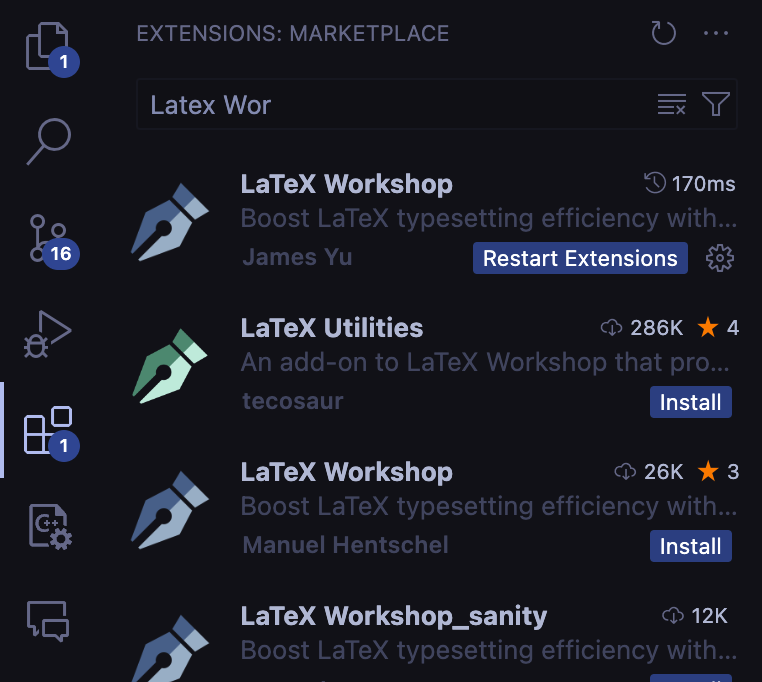
\includegraphics[width = 0.4\textwidth]{Extensions.png}
    \caption{The extension you want to install is the topmost one on the search results (the one by James Yu), which I have already installed in this image.}
\end{figure}

From here, you can simply create TeX files in VSCode by ending a file with the \verb|.tex| extension, and edit and compile them through the build button in the LaTeX Workshop sidebar tab, or the build button on top of the currently open TeX file. You can then use the LaTeX workshop sidebar once more to view the output PDF. Alternatively, you may find the output PDF in your file path and open it to the side in VSCode like you would a secondary tab of code. Nominally, this output PDF is in the same directory as your main TeX file. This is shown in \cref{fig:workspace}

\begin{figure}[ht!]
    \centering
    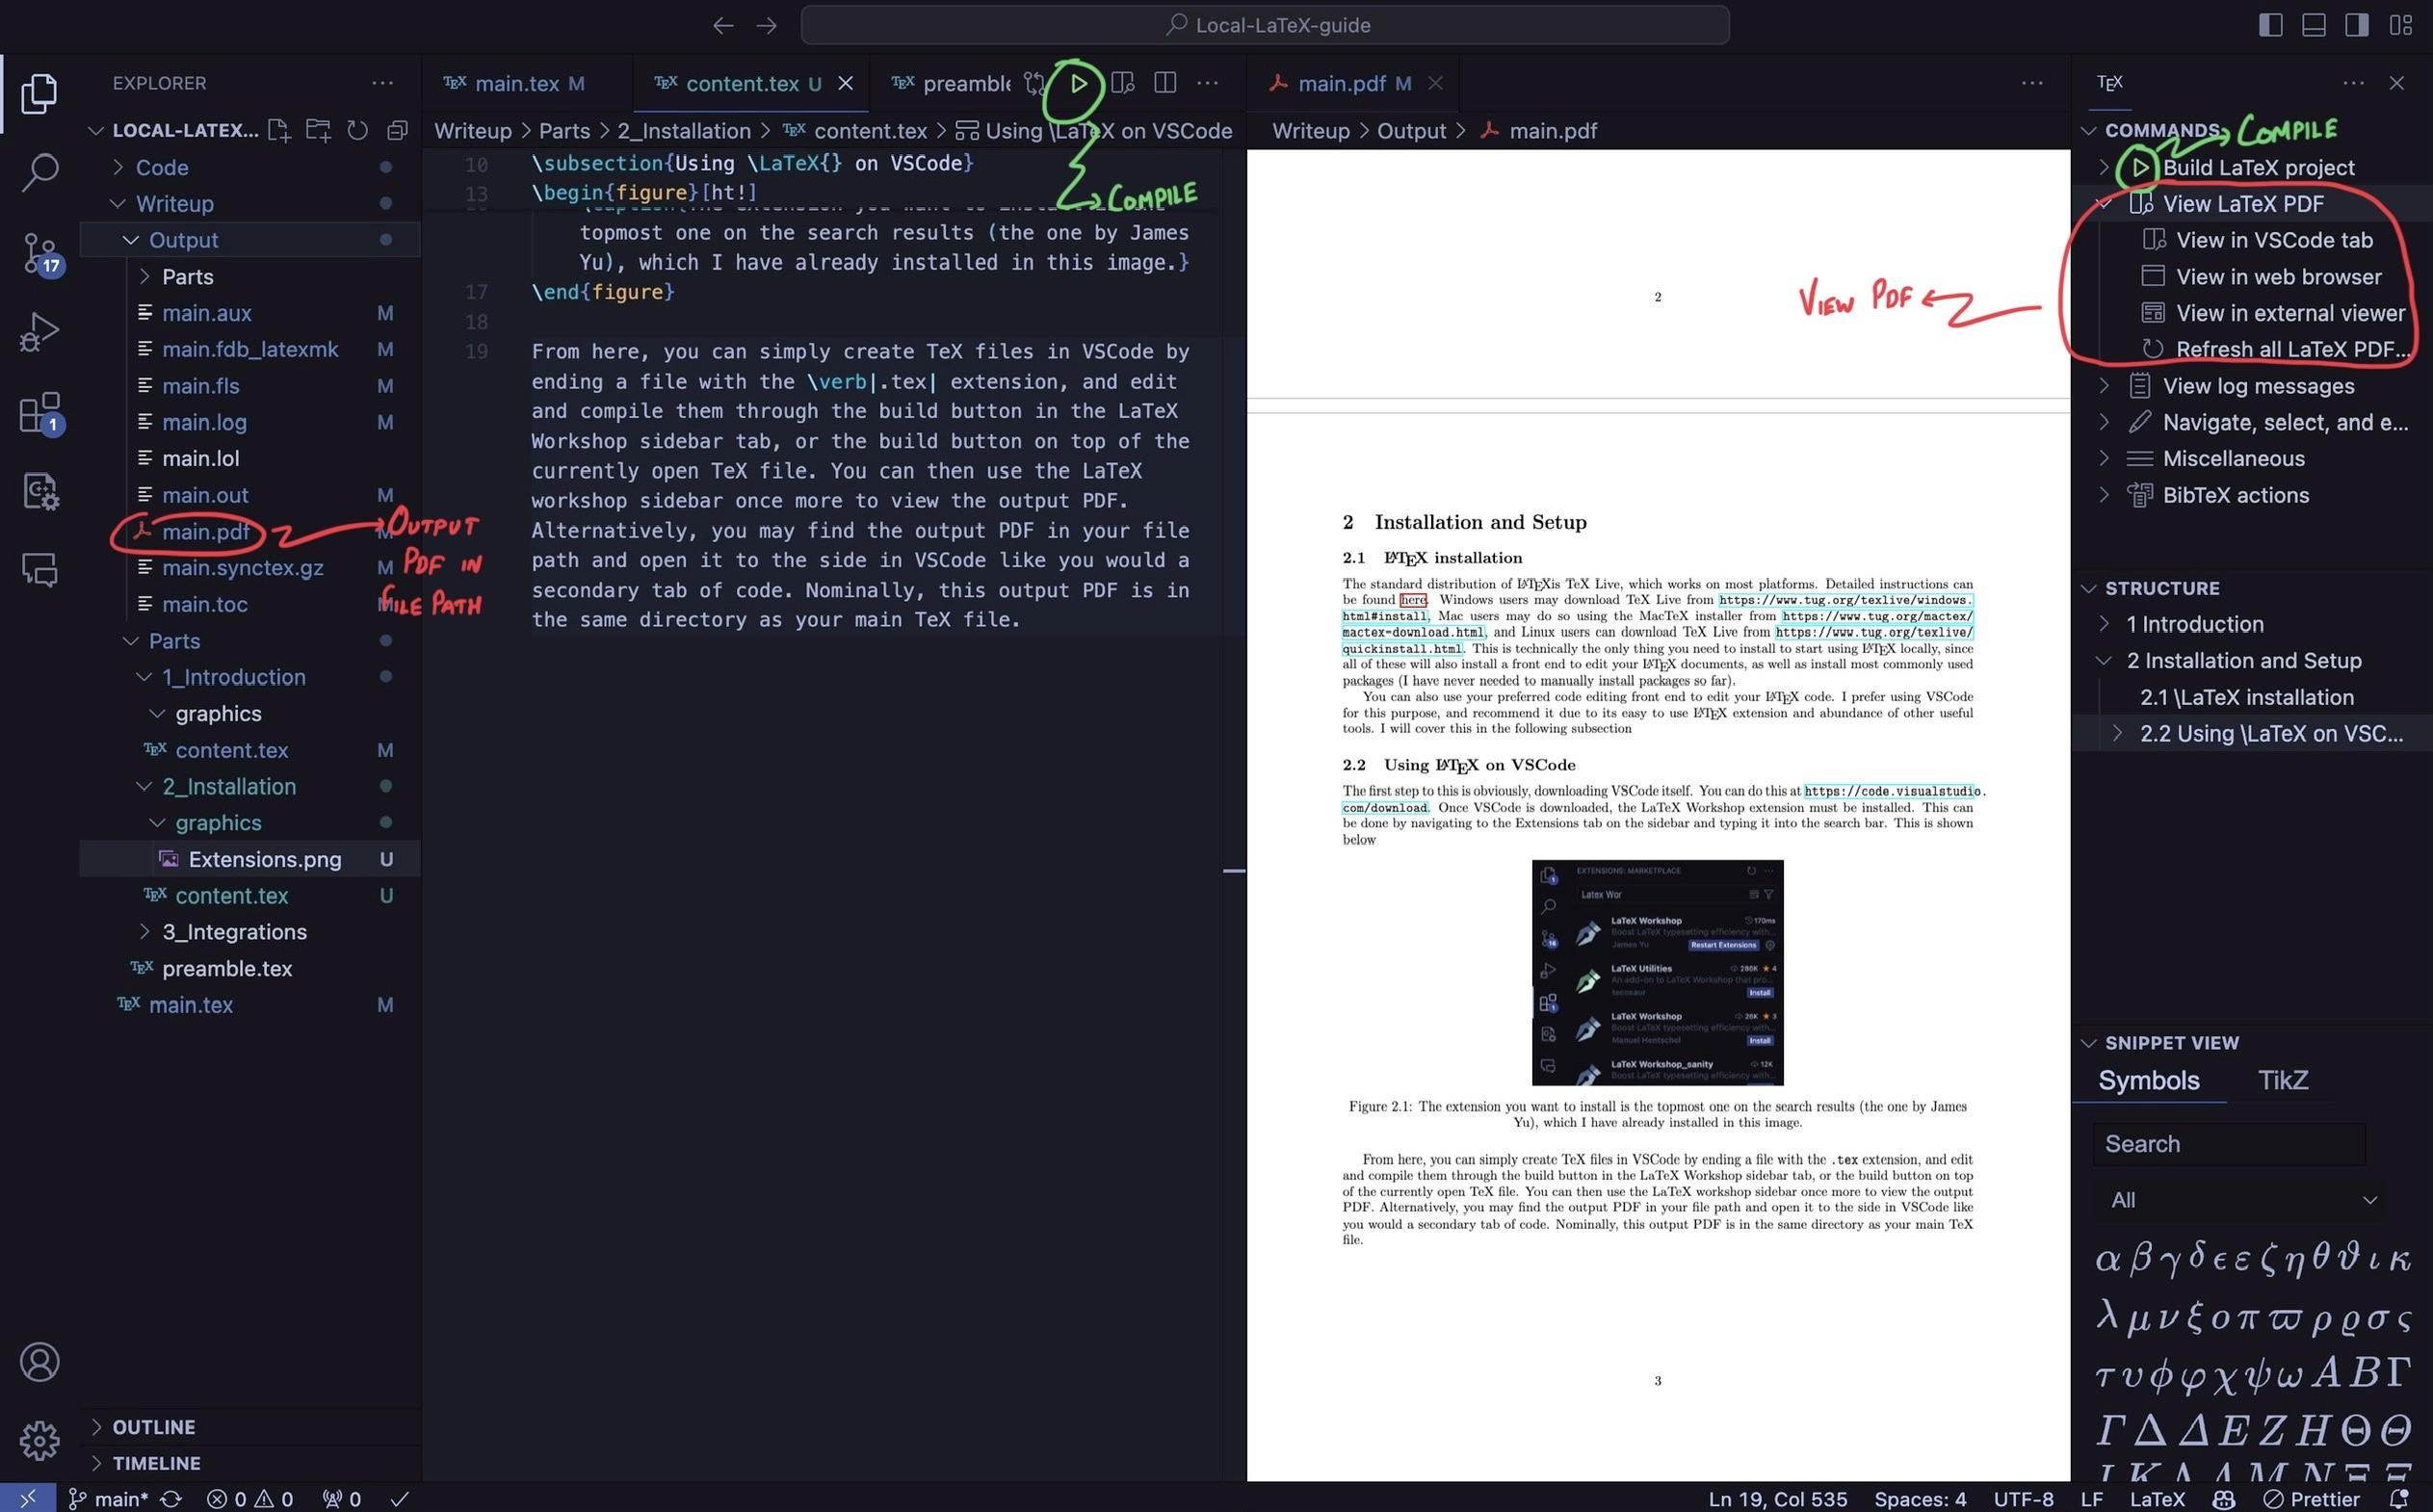
\includegraphics[width = \textwidth]{workspace.jpg}
    \caption{Where to find the output pdf and compile button in VSCode. Note that I moved the LaTeX workshop menu to the right sidebar in this picture, and have slightly modified the place where the output files go (more on this in a bit).}
    \label{fig:workspace}
\end{figure}


\newpage
\subsection{Managing \LaTeX{} files locally}

As can be noticed in \cref{fig:workspace}, there are a few files you probably haven't seen in your days using overleaf. These are the auxiliary files needed to compile the output PDF, and are produced on every compilation. While LaTeX workshop has a pretty tempting cleanup feature for these files, keeping them does help with compilation speed. As such, it is better to put them into some output folder to avoid clutter. The path to which the output and auxiliary files are sent can be edited throught the outdir setting for LaTeX Workshop on VSCode, which can be navigated to through the gear icon on the VSCode sidebar. In \cref{fig:outdir} is how I have set it up, where all output files are sent to an Output folder in the same path as \verb|main.tex|.
\begin{figure}[ht!]
    \centering
    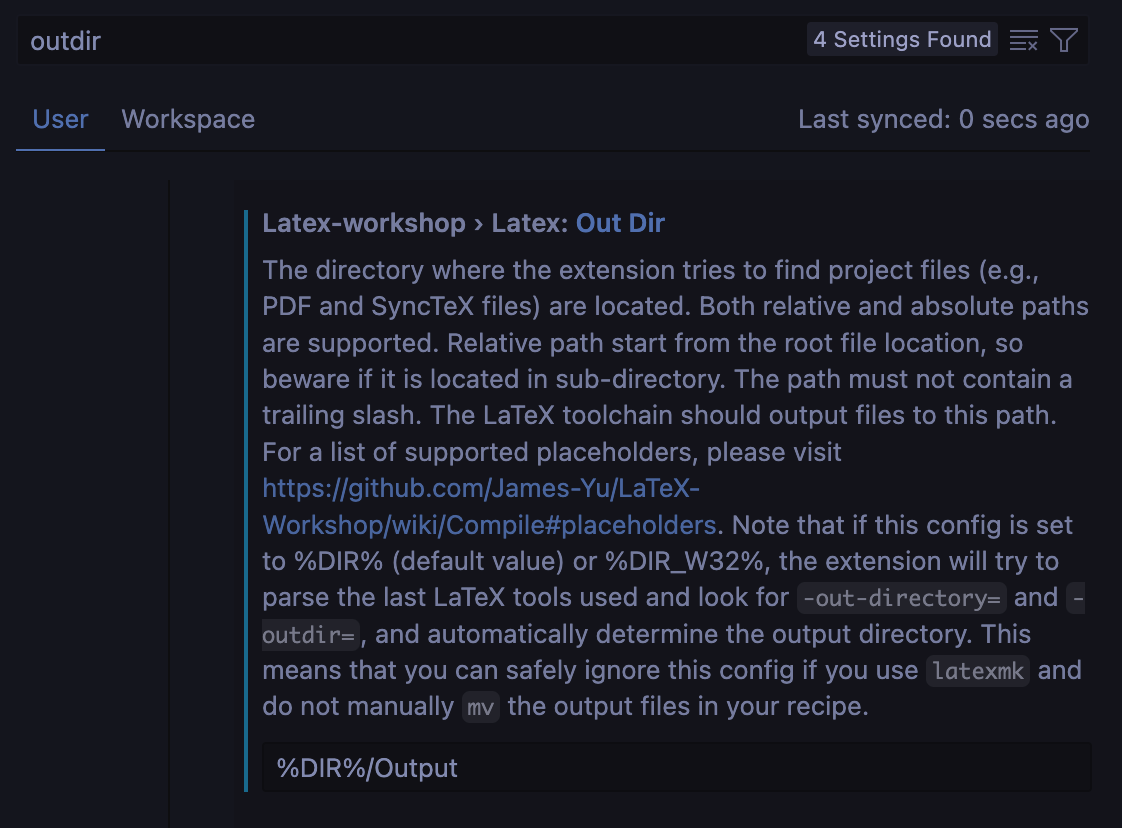
\includegraphics[width = 0.7\textwidth]{outdir.png}
    \caption{Output directory setting}
    \label{fig:outdir}
\end{figure}

Note that apart from this, I have also divided my latex document into individual files, which I am then inputting into the main file using \verb|\input{}|. Especially when dealing with local \LaTeX{}, this is preferred to \verb|\subfile{}| since the latter will make its own output folder and associated files for each subfile, bloating the project. 

To make sure the compiler always compiles main, a magic comment on these inputted subfiles is prudent. Such a comment simply tells the compiler to set the root file to be the main file is. This is given by \verb|% !TeX root = <root file directory>|. The comment can also be inserted through the search bar as in \cref{fig:magic} (this method also gives a nifty drop down to select the root file).
\begin{figure}[ht!]
    \centering
    
\includegraphics[width = 0.5\textwidth]{magic}
    \caption{Insert a magic comment}
    \label{fig:magic}
\end{figure}
However, to use this comment, you must also disable forcing recipe usage by typing \texttt{"latex-workshop.latex.build.forceRecipeUsage": false,} into the settings.json or setting it in the settings tab.

\newpage
\subsection{Some useful features and tips for \LaTeX{} in VSCode}
\begin{itemize}
    \item Turn on word wrapping in the VSCode editor. This can be done exclusively for \LaTeX{} through the language specific settings as follows
    \begin{figure}[ht!]
        \centering
        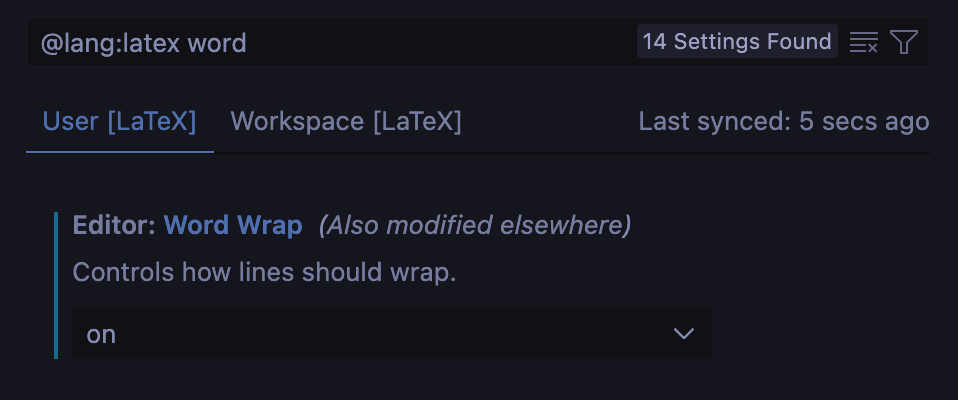
\includegraphics[width = 0.6\textwidth]{wrap}
        \caption{Word wrapping settings}
    \end{figure}
    \item Github copilot is a useful extension for some menial typesetting tasks, and especially in my experience for building tikz diagrams. Get it for free with a student github account and download it from the VSCode extensions menu, just make sure to turn off the somewhat annoying inline suggestions. This, along with the former item can be done using the following lines in settings.json (can be accessed through the VSCode searchbar)
    \begin{quote}
        \texttt{      
            "[latex]": } \{ \texttt{\\
                "editor.inlineSuggest.enabled": false,\\
                "editor.wordWrap": "on",\\
            }\},
    \end{quote}
    Additionally, editor autocompletion using copilot AI can be turned off with \texttt{"github.copilot.editor.\\enableAutoCompletions": false,}. This way, copilot won't interfere with your typing, but can still be easily accessed through a single shortcut to help do boring/repetitive tasks.

    \item LaTeX workshop supports snippets. There are several useful inbuilt ones such as \verb|BEQ| or \verb|BAL| to start equation or align environments, or \verb|@a| or \verb|@b| for greek letters like $\alpha,\beta$. A background on snippets is found on the workshop wiki at the url \url{https://github.com/James-Yu/LaTeX-Workshop/wiki/Snippets}. A concise list may also be found at \url{https://cheatography.com/jcwinkler/cheat-sheets/latex-workshop-visual-studio-code/}. You may also make custom snippets in VSCode for use by navigating to the snippets menu in the searchbar
    \begin{figure}[ht!]
        \centering
        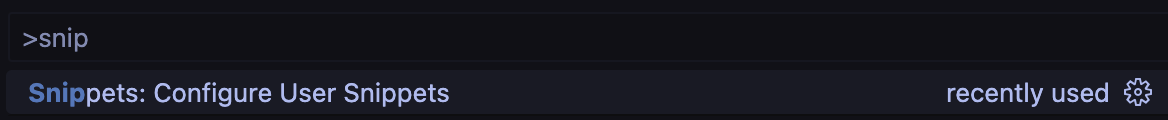
\includegraphics[width = 0.7\textwidth]{snipsnip.png}
        \caption{Snippets menu in the searchbar}
    \end{figure}
    
    \item 
    Intellisense is LaTeX workshop's capability to autofill citations, commands, environments, labels, and file names. Intellisense usually updates on file save, but you can make it update more aggressively by setting \verb|latex-workshop.intellisense.update.aggressive.enabled| to \verb|true| in the settings menu.

    \item 
    Much like double clicking the PDF in Overleaf takes you to the corresponding line of TeX, Command/Control clicking text (depending on whether the OS is Mac or Windows) in the VSCode internal PDF viewer takes you to the corresponding line of TeX. While in the TeX file, pressing Cmd+Opt+J on Mac or Ctrl+Alt+J on Windows takes you to the point in the PDF corresponding to the cursor location on the TeX file. Note that this requires the SyncTeX file to be present in the same directory as the output PDF. This file is created on each compile, and is automatically stored in the proper directory to be used.

    \item The smart clicks VSCode extension is pretty handy to select stuff in brackets. I highly recommend downloading it.
    
\end{itemize}

\subsection{Keeping your project synced}
A cool thing about using Overleaf is that since it is an online tool, it saves your progress on a cloud and can be used on basically any device. You can get cloud saving functionality using local \LaTeX{} by using any cloud based file storage such as Dropbox, OneDrive, or iCloud. However, my personal favorite for this purpose is Github due to its version control capabilities, ability to make submodules, and integration with Overleaf (to be discussed in the next section). Note that Dropbox also has this behavior with Overleaf, and this can be explored further at \url{https://www.overleaf.com/learn/how-to/Dropbox_Synchronization}. I will be showing how the Github-Overleaf integration works in the next section. 

When it comes to saving my work with Github, I essentially create a repository for entire projects, including both the code and the writeup for them. This allows me to do some cool stuff where I can easily cross reference project code in the writeup (through the listings package) and output graphics from my code directly into my writeup. Sometimes, however, it is good to save the writeup as a seperate repository within the overall project repo. A guide to creating submodules in Github is given in \url{https://gist.github.com/gitaarik/8735255}. Make sure this submodule can act as a standalone \LaTeX{} project, since that is crucial if you want to integrate the submodule with Overleaf (which will be elaborated upon in the next section).


Both my user settings .json file and user generated snippets .json file are included in the Github of this project for further reference. Additionally, the entire \LaTeX{} file tree for this document is also on the Github repo.

